\documentclass[]{article}
\usepackage{lmodern}
\usepackage{amssymb,amsmath}
\usepackage{ifxetex,ifluatex}
\usepackage{fixltx2e} % provides \textsubscript
\ifnum 0\ifxetex 1\fi\ifluatex 1\fi=0 % if pdftex
  \usepackage[T1]{fontenc}
  \usepackage[utf8]{inputenc}
\else % if luatex or xelatex
  \ifxetex
    \usepackage{mathspec}
  \else
    \usepackage{fontspec}
  \fi
  \defaultfontfeatures{Ligatures=TeX,Scale=MatchLowercase}
\fi
% use upquote if available, for straight quotes in verbatim environments
\IfFileExists{upquote.sty}{\usepackage{upquote}}{}
% use microtype if available
\IfFileExists{microtype.sty}{%
\usepackage{microtype}
\UseMicrotypeSet[protrusion]{basicmath} % disable protrusion for tt fonts
}{}
\usepackage[margin=1in]{geometry}
\usepackage{hyperref}
\PassOptionsToPackage{usenames,dvipsnames}{color} % color is loaded by hyperref
\hypersetup{unicode=true,
            pdftitle={Module 9: Recommended Exercises},
            pdfauthor={Stefanie Muff, Department of Mathematical Sciences, NTNU},
            colorlinks=true,
            linkcolor=Maroon,
            citecolor=Blue,
            urlcolor=blue,
            breaklinks=true}
\urlstyle{same}  % don't use monospace font for urls
\usepackage{color}
\usepackage{fancyvrb}
\newcommand{\VerbBar}{|}
\newcommand{\VERB}{\Verb[commandchars=\\\{\}]}
\DefineVerbatimEnvironment{Highlighting}{Verbatim}{commandchars=\\\{\}}
% Add ',fontsize=\small' for more characters per line
\usepackage{framed}
\definecolor{shadecolor}{RGB}{248,248,248}
\newenvironment{Shaded}{\begin{snugshade}}{\end{snugshade}}
\newcommand{\KeywordTok}[1]{\textcolor[rgb]{0.13,0.29,0.53}{\textbf{#1}}}
\newcommand{\DataTypeTok}[1]{\textcolor[rgb]{0.13,0.29,0.53}{#1}}
\newcommand{\DecValTok}[1]{\textcolor[rgb]{0.00,0.00,0.81}{#1}}
\newcommand{\BaseNTok}[1]{\textcolor[rgb]{0.00,0.00,0.81}{#1}}
\newcommand{\FloatTok}[1]{\textcolor[rgb]{0.00,0.00,0.81}{#1}}
\newcommand{\ConstantTok}[1]{\textcolor[rgb]{0.00,0.00,0.00}{#1}}
\newcommand{\CharTok}[1]{\textcolor[rgb]{0.31,0.60,0.02}{#1}}
\newcommand{\SpecialCharTok}[1]{\textcolor[rgb]{0.00,0.00,0.00}{#1}}
\newcommand{\StringTok}[1]{\textcolor[rgb]{0.31,0.60,0.02}{#1}}
\newcommand{\VerbatimStringTok}[1]{\textcolor[rgb]{0.31,0.60,0.02}{#1}}
\newcommand{\SpecialStringTok}[1]{\textcolor[rgb]{0.31,0.60,0.02}{#1}}
\newcommand{\ImportTok}[1]{#1}
\newcommand{\CommentTok}[1]{\textcolor[rgb]{0.56,0.35,0.01}{\textit{#1}}}
\newcommand{\DocumentationTok}[1]{\textcolor[rgb]{0.56,0.35,0.01}{\textbf{\textit{#1}}}}
\newcommand{\AnnotationTok}[1]{\textcolor[rgb]{0.56,0.35,0.01}{\textbf{\textit{#1}}}}
\newcommand{\CommentVarTok}[1]{\textcolor[rgb]{0.56,0.35,0.01}{\textbf{\textit{#1}}}}
\newcommand{\OtherTok}[1]{\textcolor[rgb]{0.56,0.35,0.01}{#1}}
\newcommand{\FunctionTok}[1]{\textcolor[rgb]{0.00,0.00,0.00}{#1}}
\newcommand{\VariableTok}[1]{\textcolor[rgb]{0.00,0.00,0.00}{#1}}
\newcommand{\ControlFlowTok}[1]{\textcolor[rgb]{0.13,0.29,0.53}{\textbf{#1}}}
\newcommand{\OperatorTok}[1]{\textcolor[rgb]{0.81,0.36,0.00}{\textbf{#1}}}
\newcommand{\BuiltInTok}[1]{#1}
\newcommand{\ExtensionTok}[1]{#1}
\newcommand{\PreprocessorTok}[1]{\textcolor[rgb]{0.56,0.35,0.01}{\textit{#1}}}
\newcommand{\AttributeTok}[1]{\textcolor[rgb]{0.77,0.63,0.00}{#1}}
\newcommand{\RegionMarkerTok}[1]{#1}
\newcommand{\InformationTok}[1]{\textcolor[rgb]{0.56,0.35,0.01}{\textbf{\textit{#1}}}}
\newcommand{\WarningTok}[1]{\textcolor[rgb]{0.56,0.35,0.01}{\textbf{\textit{#1}}}}
\newcommand{\AlertTok}[1]{\textcolor[rgb]{0.94,0.16,0.16}{#1}}
\newcommand{\ErrorTok}[1]{\textcolor[rgb]{0.64,0.00,0.00}{\textbf{#1}}}
\newcommand{\NormalTok}[1]{#1}
\usepackage{graphicx,grffile}
\makeatletter
\def\maxwidth{\ifdim\Gin@nat@width>\linewidth\linewidth\else\Gin@nat@width\fi}
\def\maxheight{\ifdim\Gin@nat@height>\textheight\textheight\else\Gin@nat@height\fi}
\makeatother
% Scale images if necessary, so that they will not overflow the page
% margins by default, and it is still possible to overwrite the defaults
% using explicit options in \includegraphics[width, height, ...]{}
\setkeys{Gin}{width=\maxwidth,height=\maxheight,keepaspectratio}
\IfFileExists{parskip.sty}{%
\usepackage{parskip}
}{% else
\setlength{\parindent}{0pt}
\setlength{\parskip}{6pt plus 2pt minus 1pt}
}
\setlength{\emergencystretch}{3em}  % prevent overfull lines
\providecommand{\tightlist}{%
  \setlength{\itemsep}{0pt}\setlength{\parskip}{0pt}}
\setcounter{secnumdepth}{0}
% Redefines (sub)paragraphs to behave more like sections
\ifx\paragraph\undefined\else
\let\oldparagraph\paragraph
\renewcommand{\paragraph}[1]{\oldparagraph{#1}\mbox{}}
\fi
\ifx\subparagraph\undefined\else
\let\oldsubparagraph\subparagraph
\renewcommand{\subparagraph}[1]{\oldsubparagraph{#1}\mbox{}}
\fi

%%% Use protect on footnotes to avoid problems with footnotes in titles
\let\rmarkdownfootnote\footnote%
\def\footnote{\protect\rmarkdownfootnote}

%%% Change title format to be more compact
\usepackage{titling}

% Create subtitle command for use in maketitle
\providecommand{\subtitle}[1]{
  \posttitle{
    \begin{center}\large#1\end{center}
    }
}

\setlength{\droptitle}{-2em}

  \title{Module 9: Recommended Exercises}
    \pretitle{\vspace{\droptitle}\centering\huge}
  \posttitle{\par}
  \subtitle{TMA4268 Statistical Learning V2020}
  \author{Stefanie Muff, Department of Mathematical Sciences, NTNU}
    \preauthor{\centering\large\emph}
  \postauthor{\par}
      \predate{\centering\large\emph}
  \postdate{\par}
    \date{March xx, 2020}


\begin{document}
\maketitle

{
\hypersetup{linkcolor=black}
\setcounter{tocdepth}{2}
\tableofcontents
}
\begin{center}\rule{0.5\linewidth}{\linethickness}\end{center}

\section{Recommended exercises}\label{recommended-exercises}

\subsection{1. Understanding the
algorithms:}\label{understanding-the-algorithms}

\begin{itemize}
\tightlist
\item
  Exercise 1, 2 and 3 in the book.
\end{itemize}

\subsection{2. Data analysis}\label{data-analysis}

\begin{itemize}
\item
  Go back and read in the \texttt{forest1} data (is located in the same
  place as \texttt{forest2}) and run the \texttt{svm} with a very high
  value for \texttt{cost}. The \texttt{forest1} is a separable problem.
\item
  Linear version of SVM: Making nicer plots for SVM from
  \href{https://www.youtube.com/watch?v=qhyyufR0930\&list=PL5-da3qGB5IDl6MkmovVdZwyYOhpCxo5o\&index=5}{Lab
  video}. Go through the code and see what is happening (and see the
  video if you want more explanation).
\end{itemize}

\begin{Shaded}
\begin{Highlighting}[]
\CommentTok{# code taken from video by Trevor Hastie linked above}
\KeywordTok{library}\NormalTok{(e1071)}
\CommentTok{# fake data}
\KeywordTok{set.seed}\NormalTok{(}\DecValTok{10111}\NormalTok{)}
\NormalTok{x =}\StringTok{ }\KeywordTok{matrix}\NormalTok{(}\KeywordTok{rnorm}\NormalTok{(}\DecValTok{40}\NormalTok{), }\DecValTok{20}\NormalTok{, }\DecValTok{2}\NormalTok{)}
\NormalTok{y =}\StringTok{ }\KeywordTok{rep}\NormalTok{(}\KeywordTok{c}\NormalTok{(}\OperatorTok{-}\DecValTok{1}\NormalTok{, }\DecValTok{1}\NormalTok{), }\KeywordTok{c}\NormalTok{(}\DecValTok{10}\NormalTok{, }\DecValTok{10}\NormalTok{))}
\NormalTok{x[y }\OperatorTok{==}\StringTok{ }\DecValTok{1}\NormalTok{, ] =}\StringTok{ }\NormalTok{x[y }\OperatorTok{==}\StringTok{ }\DecValTok{1}\NormalTok{, ] }\OperatorTok{+}\StringTok{ }\DecValTok{1}
\KeywordTok{plot}\NormalTok{(x, }\DataTypeTok{col =}\NormalTok{ y }\OperatorTok{+}\StringTok{ }\DecValTok{3}\NormalTok{, }\DataTypeTok{pch =} \DecValTok{19}\NormalTok{)}
\end{Highlighting}
\end{Shaded}

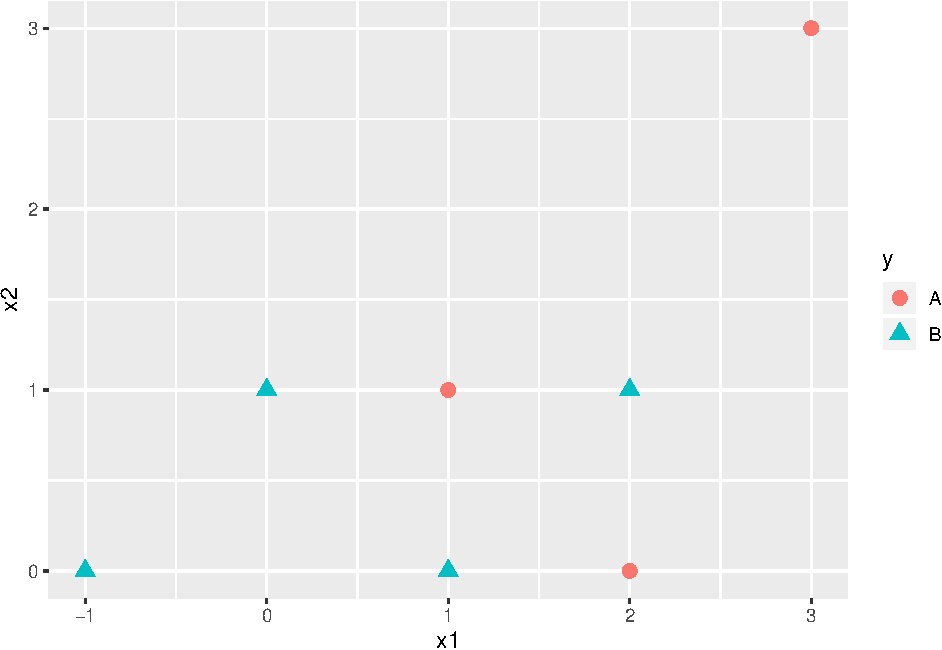
\includegraphics{RecEx9_files/figure-latex/unnamed-chunk-1-1.pdf}

\begin{Shaded}
\begin{Highlighting}[]
\CommentTok{# calling svm}
\NormalTok{dat =}\StringTok{ }\KeywordTok{data.frame}\NormalTok{(x, }\DataTypeTok{y =} \KeywordTok{as.factor}\NormalTok{(y))}
\NormalTok{svmfit =}\StringTok{ }\KeywordTok{svm}\NormalTok{(y }\OperatorTok{~}\StringTok{ }\NormalTok{., }\DataTypeTok{data =}\NormalTok{ dat, }\DataTypeTok{kernel =} \StringTok{"linear"}\NormalTok{, }\DataTypeTok{cost =} \DecValTok{10}\NormalTok{, }\DataTypeTok{scale =} \OtherTok{FALSE}\NormalTok{)}
\KeywordTok{print}\NormalTok{(svmfit)}
\end{Highlighting}
\end{Shaded}

\begin{verbatim}
## 
## Call:
## svm(formula = y ~ ., data = dat, kernel = "linear", cost = 10, 
##     scale = FALSE)
## 
## 
## Parameters:
##    SVM-Type:  C-classification 
##  SVM-Kernel:  linear 
##        cost:  10 
## 
## Number of Support Vectors:  6
\end{verbatim}

\begin{Shaded}
\begin{Highlighting}[]
\CommentTok{# grid for plotting}
\NormalTok{make.grid =}\StringTok{ }\ControlFlowTok{function}\NormalTok{(x, }\DataTypeTok{n =} \DecValTok{75}\NormalTok{) \{}
\NormalTok{    grange =}\StringTok{ }\KeywordTok{apply}\NormalTok{(x, }\DecValTok{2}\NormalTok{, range)}
\NormalTok{    x1 =}\StringTok{ }\KeywordTok{seq}\NormalTok{(}\DataTypeTok{from =}\NormalTok{ grange[}\DecValTok{1}\NormalTok{, }\DecValTok{1}\NormalTok{], }\DataTypeTok{to =}\NormalTok{ grange[}\DecValTok{2}\NormalTok{, }\DecValTok{1}\NormalTok{], }\DataTypeTok{length =}\NormalTok{ n)}
\NormalTok{    x2 =}\StringTok{ }\KeywordTok{seq}\NormalTok{(}\DataTypeTok{from =}\NormalTok{ grange[}\DecValTok{1}\NormalTok{, }\DecValTok{2}\NormalTok{], }\DataTypeTok{to =}\NormalTok{ grange[}\DecValTok{2}\NormalTok{, }\DecValTok{2}\NormalTok{], }\DataTypeTok{length =}\NormalTok{ n)}
    \KeywordTok{expand.grid}\NormalTok{(}\DataTypeTok{X1 =}\NormalTok{ x1, }\DataTypeTok{X2 =}\NormalTok{ x2)}
\NormalTok{\}}
\NormalTok{xgrid =}\StringTok{ }\KeywordTok{make.grid}\NormalTok{(x)}
\NormalTok{ygrid =}\StringTok{ }\KeywordTok{predict}\NormalTok{(svmfit, xgrid)}
\KeywordTok{plot}\NormalTok{(xgrid, }\DataTypeTok{col =} \KeywordTok{c}\NormalTok{(}\StringTok{"red"}\NormalTok{, }\StringTok{"blue"}\NormalTok{)[}\KeywordTok{as.numeric}\NormalTok{(ygrid)], }\DataTypeTok{pch =} \DecValTok{20}\NormalTok{, }\DataTypeTok{cex =} \FloatTok{0.2}\NormalTok{)}
\KeywordTok{points}\NormalTok{(x, }\DataTypeTok{col =}\NormalTok{ y }\OperatorTok{+}\StringTok{ }\DecValTok{3}\NormalTok{, }\DataTypeTok{pch =} \DecValTok{19}\NormalTok{)}
\KeywordTok{points}\NormalTok{(x[svmfit}\OperatorTok{$}\NormalTok{index, ], }\DataTypeTok{pch =} \DecValTok{5}\NormalTok{, }\DataTypeTok{cex =} \DecValTok{2}\NormalTok{)}
\end{Highlighting}
\end{Shaded}

\includegraphics{RecEx9_files/figure-latex/unnamed-chunk-1-2.pdf}

\begin{Shaded}
\begin{Highlighting}[]
\CommentTok{# more info on results - class boundary}

\NormalTok{beta =}\StringTok{ }\KeywordTok{drop}\NormalTok{(}\KeywordTok{t}\NormalTok{(svmfit}\OperatorTok{$}\NormalTok{coefs) }\OperatorTok\StringTok{ }\NormalTok{x[svmfit}\OperatorTok{$}\NormalTok{index, ])}
\NormalTok{beta0 =}\StringTok{ }\NormalTok{svmfit}\OperatorTok{$}\NormalTok{rho}
\KeywordTok{plot}\NormalTok{(xgrid, }\DataTypeTok{col =} \KeywordTok{c}\NormalTok{(}\StringTok{"red"}\NormalTok{, }\StringTok{"blue"}\NormalTok{)[}\KeywordTok{as.numeric}\NormalTok{(ygrid)], }\DataTypeTok{pch =} \DecValTok{20}\NormalTok{, }\DataTypeTok{cex =} \FloatTok{0.2}\NormalTok{)}
\KeywordTok{points}\NormalTok{(x, }\DataTypeTok{col =}\NormalTok{ y }\OperatorTok{+}\StringTok{ }\DecValTok{3}\NormalTok{, }\DataTypeTok{pch =} \DecValTok{19}\NormalTok{)}
\KeywordTok{points}\NormalTok{(x[svmfit}\OperatorTok{$}\NormalTok{index, ], }\DataTypeTok{pch =} \DecValTok{5}\NormalTok{, }\DataTypeTok{cex =} \DecValTok{2}\NormalTok{)}
\KeywordTok{abline}\NormalTok{(beta0}\OperatorTok{/}\NormalTok{beta[}\DecValTok{2}\NormalTok{], }\OperatorTok{-}\NormalTok{beta[}\DecValTok{1}\NormalTok{]}\OperatorTok{/}\NormalTok{beta[}\DecValTok{2}\NormalTok{])  }\CommentTok{#class boundary}
\KeywordTok{abline}\NormalTok{((beta0 }\OperatorTok{-}\StringTok{ }\DecValTok{1}\NormalTok{)}\OperatorTok{/}\NormalTok{beta[}\DecValTok{2}\NormalTok{], }\OperatorTok{-}\NormalTok{beta[}\DecValTok{1}\NormalTok{]}\OperatorTok{/}\NormalTok{beta[}\DecValTok{2}\NormalTok{])  }\CommentTok{#class boundary-margin}
\KeywordTok{abline}\NormalTok{((beta0 }\OperatorTok{+}\StringTok{ }\DecValTok{1}\NormalTok{)}\OperatorTok{/}\NormalTok{beta[}\DecValTok{2}\NormalTok{], }\OperatorTok{-}\NormalTok{beta[}\DecValTok{1}\NormalTok{]}\OperatorTok{/}\NormalTok{beta[}\DecValTok{2}\NormalTok{])  }\CommentTok{#class boundary+margin}
\end{Highlighting}
\end{Shaded}

\includegraphics{RecEx9_files/figure-latex/unnamed-chunk-1-3.pdf}

\begin{itemize}
\tightlist
\item
  SVM for non-linear class boundary using simulated data set from @ESL
  where the truth is known (mixtures of normals probably).
\end{itemize}

\begin{Shaded}
\begin{Highlighting}[]
\KeywordTok{load}\NormalTok{(}\KeywordTok{url}\NormalTok{(}\StringTok{"https://web.stanford.edu/~hastie/ElemStatLearn/datasets/ESL.mixture.rda"}\NormalTok{))}
\KeywordTok{names}\NormalTok{(ESL.mixture)}
\end{Highlighting}
\end{Shaded}

\begin{verbatim}
## [1] "x"        "y"        "xnew"     "prob"     "marginal" "px1"     
## [7] "px2"      "means"
\end{verbatim}

\begin{Shaded}
\begin{Highlighting}[]
\KeywordTok{rm}\NormalTok{(x, y)}
\KeywordTok{attach}\NormalTok{(ESL.mixture)}

\KeywordTok{plot}\NormalTok{(x, }\DataTypeTok{col =}\NormalTok{ y }\OperatorTok{+}\StringTok{ }\DecValTok{1}\NormalTok{)}
\end{Highlighting}
\end{Shaded}

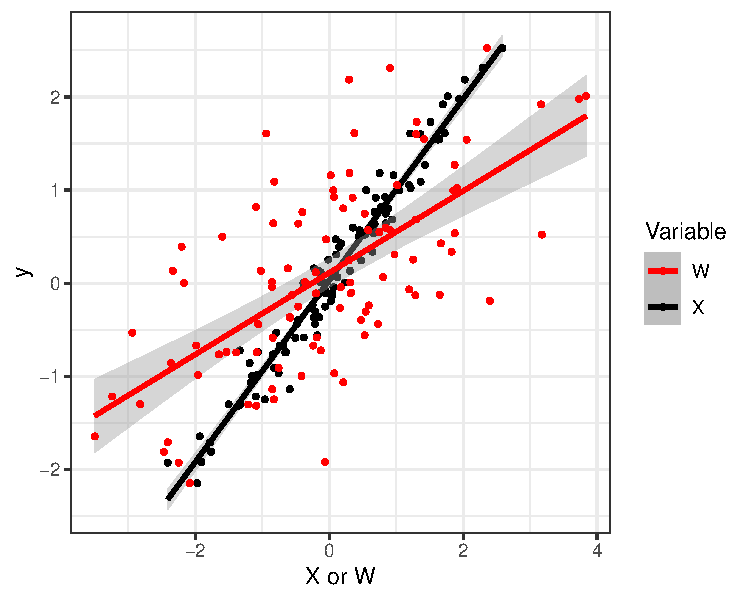
\includegraphics{RecEx9_files/figure-latex/unnamed-chunk-2-1.pdf}

\begin{Shaded}
\begin{Highlighting}[]
\NormalTok{dat =}\StringTok{ }\KeywordTok{data.frame}\NormalTok{(}\DataTypeTok{y =} \KeywordTok{factor}\NormalTok{(y), x)}
\NormalTok{fit =}\StringTok{ }\KeywordTok{svm}\NormalTok{(}\KeywordTok{factor}\NormalTok{(y) }\OperatorTok{~}\StringTok{ }\NormalTok{., }\DataTypeTok{data =}\NormalTok{ dat, }\DataTypeTok{scale =} \OtherTok{FALSE}\NormalTok{, }\DataTypeTok{kernel =} \StringTok{"radial"}\NormalTok{, }
    \DataTypeTok{cost =} \DecValTok{5}\NormalTok{)}

\NormalTok{xgrid =}\StringTok{ }\KeywordTok{expand.grid}\NormalTok{(}\DataTypeTok{X1 =}\NormalTok{ px1, }\DataTypeTok{X2 =}\NormalTok{ px2)}
\NormalTok{ygrid =}\StringTok{ }\KeywordTok{predict}\NormalTok{(fit, xgrid)}
\KeywordTok{plot}\NormalTok{(xgrid, }\DataTypeTok{col =} \KeywordTok{as.numeric}\NormalTok{(ygrid), }\DataTypeTok{pch =} \DecValTok{20}\NormalTok{, }\DataTypeTok{cex =} \FloatTok{0.2}\NormalTok{)}
\KeywordTok{points}\NormalTok{(x, }\DataTypeTok{col =}\NormalTok{ y }\OperatorTok{+}\StringTok{ }\DecValTok{1}\NormalTok{, }\DataTypeTok{pch =} \DecValTok{19}\NormalTok{)}

\CommentTok{# decision boundary}
\NormalTok{func =}\StringTok{ }\KeywordTok{predict}\NormalTok{(fit, xgrid, }\DataTypeTok{decision.values =} \OtherTok{TRUE}\NormalTok{)}
\NormalTok{func =}\StringTok{ }\KeywordTok{attributes}\NormalTok{(func)}\OperatorTok{$}\NormalTok{decision}
\KeywordTok{contour}\NormalTok{(px1, px2, }\KeywordTok{matrix}\NormalTok{(func, }\DecValTok{69}\NormalTok{, }\DecValTok{99}\NormalTok{), }\DataTypeTok{level =} \DecValTok{0}\NormalTok{, }\DataTypeTok{add =} \OtherTok{TRUE}\NormalTok{)  }\CommentTok{#svm boundary}
\KeywordTok{contour}\NormalTok{(px1, px2, }\KeywordTok{matrix}\NormalTok{(prob, }\DecValTok{69}\NormalTok{, }\DecValTok{99}\NormalTok{), }\DataTypeTok{level =} \FloatTok{0.5}\NormalTok{, }\DataTypeTok{add =} \OtherTok{TRUE}\NormalTok{, }\DataTypeTok{col =} \StringTok{"blue"}\NormalTok{, }
    \DataTypeTok{lwd =} \DecValTok{2}\NormalTok{)  }\CommentTok{#truth}
\end{Highlighting}
\end{Shaded}

\includegraphics{RecEx9_files/figure-latex/unnamed-chunk-2-2.pdf}

\subsection{Compulsory exercise 3 2018: Problem 2 - Nonlinear class
boundaries and support vector
machine}\label{compulsory-exercise-3-2018-problem-2---nonlinear-class-boundaries-and-support-vector-machine}

\subsection{3 a) Bayes decision boundary {[}1
point{]}}\label{a-bayes-decision-boundary-1-point}

We will study classification applied to a simulated data set with two
classes from @ESL, where the data set is supplied together with the
Bayes decision boundary. The boundary is plotted below, together with a
training set.

\begin{Shaded}
\begin{Highlighting}[]
\KeywordTok{load}\NormalTok{(}\KeywordTok{url}\NormalTok{(}\StringTok{"https://web.stanford.edu/~hastie/ElemStatLearn/datasets/ESL.mixture.rda"}\NormalTok{))}
\CommentTok{# names(ESL.mixture) prob gives probabilites for each class when the}
\CommentTok{# true density functions are known px1 and px2 are coordinates in x1}
\CommentTok{# (length 69) and x2 (length 99) where class probabilites are}
\CommentTok{# calculated}
\KeywordTok{rm}\NormalTok{(x, y)}
\KeywordTok{attach}\NormalTok{(ESL.mixture)}
\NormalTok{dat =}\StringTok{ }\KeywordTok{data.frame}\NormalTok{(}\DataTypeTok{y =} \KeywordTok{factor}\NormalTok{(y), x)}
\NormalTok{xgrid =}\StringTok{ }\KeywordTok{expand.grid}\NormalTok{(}\DataTypeTok{X1 =}\NormalTok{ px1, }\DataTypeTok{X2 =}\NormalTok{ px2)}
\KeywordTok{par}\NormalTok{(}\DataTypeTok{pty =} \StringTok{"s"}\NormalTok{)}
\KeywordTok{plot}\NormalTok{(xgrid, }\DataTypeTok{pch =} \DecValTok{20}\NormalTok{, }\DataTypeTok{cex =} \FloatTok{0.2}\NormalTok{)}
\KeywordTok{points}\NormalTok{(x, }\DataTypeTok{col =}\NormalTok{ y }\OperatorTok{+}\StringTok{ }\DecValTok{1}\NormalTok{, }\DataTypeTok{pch =} \DecValTok{20}\NormalTok{)}
\KeywordTok{contour}\NormalTok{(px1, px2, }\KeywordTok{matrix}\NormalTok{(prob, }\DecValTok{69}\NormalTok{, }\DecValTok{99}\NormalTok{), }\DataTypeTok{level =} \FloatTok{0.5}\NormalTok{, }\DataTypeTok{add =} \OtherTok{TRUE}\NormalTok{, }\DataTypeTok{col =} \StringTok{"blue"}\NormalTok{, }
    \DataTypeTok{lwd =} \DecValTok{2}\NormalTok{)  }\CommentTok{#optimal boundary}
\end{Highlighting}
\end{Shaded}

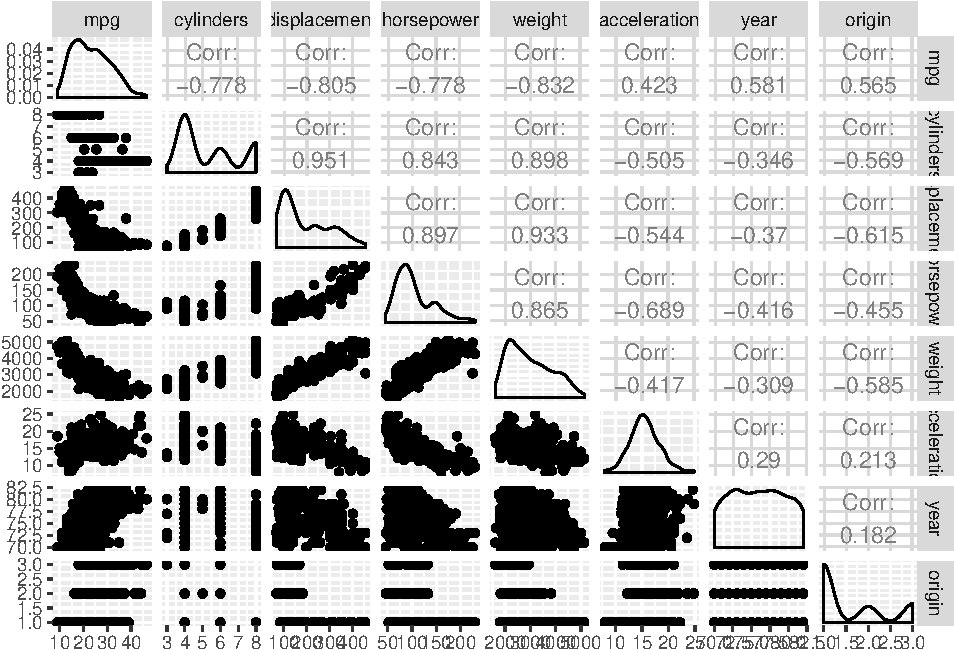
\includegraphics{RecEx9_files/figure-latex/unnamed-chunk-3-1.pdf}

\begin{itemize}
\tightlist
\item
  Q11. What is a Bayes classifier, Bayes decision boundary and Bayes
  error rate? Hint: pages 37-39 in @ISL.
\item
  Q12. When the Bayes decision boundary is known, do we then need a test
  set?
\end{itemize}

\subsubsection{b) Support vector machine {[}1
point{]}}\label{b-support-vector-machine-1-point}

\begin{Shaded}
\begin{Highlighting}[]
\KeywordTok{library}\NormalTok{(e1071)}
\CommentTok{# support vector classifier}
\NormalTok{svcfits =}\StringTok{ }\KeywordTok{tune}\NormalTok{(svm, }\KeywordTok{factor}\NormalTok{(y) }\OperatorTok{~}\StringTok{ }\NormalTok{., }\DataTypeTok{data =}\NormalTok{ dat, }\DataTypeTok{scale =} \OtherTok{FALSE}\NormalTok{, }\DataTypeTok{kernel =} \StringTok{"linear"}\NormalTok{, }
    \DataTypeTok{ranges =} \KeywordTok{list}\NormalTok{(}\DataTypeTok{cost =} \KeywordTok{c}\NormalTok{(}\FloatTok{0.01}\NormalTok{, }\FloatTok{0.1}\NormalTok{, }\DecValTok{1}\NormalTok{, }\DecValTok{5}\NormalTok{, }\DecValTok{10}\NormalTok{)))}
\KeywordTok{summary}\NormalTok{(svcfits)}
\end{Highlighting}
\end{Shaded}

\begin{verbatim}
## 
## Parameter tuning of 'svm':
## 
## - sampling method: 10-fold cross validation 
## 
## - best parameters:
##  cost
##  0.01
## 
## - best performance: 0.27 
## 
## - Detailed performance results:
##    cost error dispersion
## 1  0.01 0.270 0.11595018
## 2  0.10 0.290 0.07745967
## 3  1.00 0.295 0.07619420
## 4  5.00 0.295 0.07619420
## 5 10.00 0.300 0.07817360
\end{verbatim}

\begin{Shaded}
\begin{Highlighting}[]
\NormalTok{svcfit =}\StringTok{ }\KeywordTok{svm}\NormalTok{(}\KeywordTok{factor}\NormalTok{(y) }\OperatorTok{~}\StringTok{ }\NormalTok{., }\DataTypeTok{data =}\NormalTok{ dat, }\DataTypeTok{scale =} \OtherTok{FALSE}\NormalTok{, }\DataTypeTok{kernel =} \StringTok{"linear"}\NormalTok{, }
    \DataTypeTok{cost =} \FloatTok{0.01}\NormalTok{)}
\CommentTok{# support vector machine with radial kernel}
\KeywordTok{set.seed}\NormalTok{(}\DecValTok{4268}\NormalTok{)}
\NormalTok{svmfits =}\StringTok{ }\KeywordTok{tune}\NormalTok{(svm, }\KeywordTok{factor}\NormalTok{(y) }\OperatorTok{~}\StringTok{ }\NormalTok{., }\DataTypeTok{data =}\NormalTok{ dat, }\DataTypeTok{scale =} \OtherTok{FALSE}\NormalTok{, }\DataTypeTok{kernel =} \StringTok{"radial"}\NormalTok{, }
    \DataTypeTok{ranges =} \KeywordTok{list}\NormalTok{(}\DataTypeTok{cost =} \KeywordTok{c}\NormalTok{(}\FloatTok{0.01}\NormalTok{, }\FloatTok{0.1}\NormalTok{, }\DecValTok{1}\NormalTok{, }\DecValTok{5}\NormalTok{, }\DecValTok{10}\NormalTok{), }\DataTypeTok{gamma =} \KeywordTok{c}\NormalTok{(}\FloatTok{0.01}\NormalTok{, }\DecValTok{1}\NormalTok{, }\DecValTok{5}\NormalTok{, }
        \DecValTok{10}\NormalTok{)))}
\KeywordTok{summary}\NormalTok{(svmfits)}
\end{Highlighting}
\end{Shaded}

\begin{verbatim}
## 
## Parameter tuning of 'svm':
## 
## - sampling method: 10-fold cross validation 
## 
## - best parameters:
##  cost gamma
##     1     5
## 
## - best performance: 0.16 
## 
## - Detailed performance results:
##     cost gamma error dispersion
## 1   0.01  0.01 0.550 0.11547005
## 2   0.10  0.01 0.530 0.12064641
## 3   1.00  0.01 0.275 0.09204468
## 4   5.00  0.01 0.275 0.06346478
## 5  10.00  0.01 0.290 0.08432740
## 6   0.01  1.00 0.535 0.14539219
## 7   0.10  1.00 0.230 0.08232726
## 8   1.00  1.00 0.175 0.06770032
## 9   5.00  1.00 0.175 0.06770032
## 10 10.00  1.00 0.180 0.08881942
## 11  0.01  5.00 0.505 0.20608790
## 12  0.10  5.00 0.400 0.18708287
## 13  1.00  5.00 0.160 0.07745967
## 14  5.00  5.00 0.215 0.09143911
## 15 10.00  5.00 0.195 0.09559754
## 16  0.01 10.00 0.515 0.18566697
## 17  0.10 10.00 0.505 0.18173546
## 18  1.00 10.00 0.190 0.07745967
## 19  5.00 10.00 0.235 0.12483322
## 20 10.00 10.00 0.255 0.13006409
\end{verbatim}

\begin{Shaded}
\begin{Highlighting}[]
\NormalTok{svmfit =}\StringTok{ }\KeywordTok{svm}\NormalTok{(}\KeywordTok{factor}\NormalTok{(y) }\OperatorTok{~}\StringTok{ }\NormalTok{., }\DataTypeTok{data =}\NormalTok{ dat, }\DataTypeTok{scale =} \OtherTok{FALSE}\NormalTok{, }\DataTypeTok{kernel =} \StringTok{"radial"}\NormalTok{, }
    \DataTypeTok{cost =} \DecValTok{1}\NormalTok{, }\DataTypeTok{gamma =} \DecValTok{5}\NormalTok{)}

\CommentTok{# the same as in a - the Bayes boundary}
\KeywordTok{par}\NormalTok{(}\DataTypeTok{pty =} \StringTok{"s"}\NormalTok{)}
\KeywordTok{plot}\NormalTok{(xgrid, }\DataTypeTok{pch =} \DecValTok{20}\NormalTok{, }\DataTypeTok{cex =} \FloatTok{0.2}\NormalTok{)}
\KeywordTok{points}\NormalTok{(x, }\DataTypeTok{col =}\NormalTok{ y }\OperatorTok{+}\StringTok{ }\DecValTok{1}\NormalTok{, }\DataTypeTok{pch =} \DecValTok{20}\NormalTok{)}
\KeywordTok{contour}\NormalTok{(px1, px2, }\KeywordTok{matrix}\NormalTok{(prob, }\DecValTok{69}\NormalTok{, }\DecValTok{99}\NormalTok{), }\DataTypeTok{level =} \FloatTok{0.5}\NormalTok{, }\DataTypeTok{add =} \OtherTok{TRUE}\NormalTok{, }\DataTypeTok{col =} \StringTok{"blue"}\NormalTok{, }
    \DataTypeTok{lwd =} \DecValTok{2}\NormalTok{)  }\CommentTok{#optimal boundary}

\CommentTok{# decision boundaries from svc and svm added}
\NormalTok{svcfunc =}\StringTok{ }\KeywordTok{predict}\NormalTok{(svcfit, xgrid, }\DataTypeTok{decision.values =} \OtherTok{TRUE}\NormalTok{)}
\NormalTok{svcfunc =}\StringTok{ }\KeywordTok{attributes}\NormalTok{(svcfunc)}\OperatorTok{$}\NormalTok{decision}
\KeywordTok{contour}\NormalTok{(px1, px2, }\KeywordTok{matrix}\NormalTok{(svcfunc, }\DecValTok{69}\NormalTok{, }\DecValTok{99}\NormalTok{), }\DataTypeTok{level =} \DecValTok{0}\NormalTok{, }\DataTypeTok{add =} \OtherTok{TRUE}\NormalTok{, }\DataTypeTok{col =} \StringTok{"red"}\NormalTok{)  }\CommentTok{#svc boundary}
\NormalTok{svmfunc =}\StringTok{ }\KeywordTok{predict}\NormalTok{(svmfit, xgrid, }\DataTypeTok{decision.values =} \OtherTok{TRUE}\NormalTok{)}
\NormalTok{svmfunc =}\StringTok{ }\KeywordTok{attributes}\NormalTok{(svmfunc)}\OperatorTok{$}\NormalTok{decision}
\KeywordTok{contour}\NormalTok{(px1, px2, }\KeywordTok{matrix}\NormalTok{(svmfunc, }\DecValTok{69}\NormalTok{, }\DecValTok{99}\NormalTok{), }\DataTypeTok{level =} \DecValTok{0}\NormalTok{, }\DataTypeTok{add =} \OtherTok{TRUE}\NormalTok{, }\DataTypeTok{col =} \StringTok{"orange"}\NormalTok{)  }\CommentTok{#svm boundary}
\end{Highlighting}
\end{Shaded}

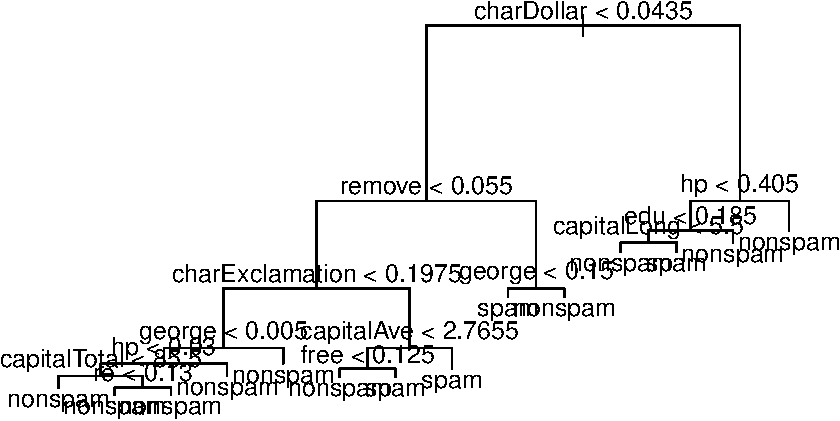
\includegraphics{RecEx9_files/figure-latex/unnamed-chunk-4-1.pdf}

\begin{itemize}
\tightlist
\item
  Q13. What is the difference between a support vector classifier and a
  support vector machine?
\item
  Q14. What are parameters for the support vector classifier and the
  support vector machine? How are these chosen above?
\item
  Q15. How would you evaluate the support vector machine decision
  boundary compared to the Bayes decision boundary?
\end{itemize}


\end{document}
